%===============================================================================
% Template stuff

\documentclass[times]{thesisMDU}
\usepackage[british,style=iso]{datetime2}  

% !!! NEEDS TO BE EDITED !!!
\fancyHeader{Multi-robot Soccer - RoboCup}{V. Eriksson et al.}
%\fancyHeader{Short title of the thesis}{Authors}

\university{Mälardalen University}
\department{School of Innovation Design and Engineering\\ Västerås, Sweden}

%===============================================================================
% Includes

%===============================================================================
% Add packages here

% QoL
\usepackage{comment}

% Fixing labels and captions for tables and figures
\usepackage{caption}

% Tables
\usepackage{tabularx}
\usepackage[table,xcdraw]{xcolor}

% Create figures and animations
\usepackage{tikz,pgfplots}
\usetikzlibrary{positioning,arrows.meta,calc}
\pgfplotsset{compat=newest}

% Linking
\usepackage{hyperref}

%===============================================================================


%===============================================================================
% Title

\subject{Project report for Project Courses in Robotics \& Intelligent embedded systems \\ Robotics \& Intelligent embedded systems 30.0 credits}
%\subject{Thesis for the Degree of Master of Science in Engineering \\ Robotics 30.0 credits}
\thesisTitle{Multi-robot Soccer - RoboCup}

%===============================================================================
% Authors

\addAuthor{Viktor Eriksson}{ven20002@student.mdu.se}
\addAuthor{Anton Grusell}{agl19003@student.mdu.se}
\addAuthor{Mudar Ibrahim}{mim20004@student.mdu.se}
\addAuthor{Jacob Johansson}{jjn20030@student.mdu.se}
\addAuthor{Aiza Aziz Khan}{akn23018@student.mdu.se}
\addAuthor{Carl Larsson}{cln20001@student.mdu.se}
\addAuthor{Johanna Melander}{jmr19002@student.mdu.se}
\addAuthor{Shruti Puthiya Kunnon}{spn23001@student.mdu.se}
\addAuthor{Pontus Svensson}{psn19003@student.mdu.se}
\addAuthor{Fredrik Westerbom}{fnl18001@student.mdu.se}
\addAuthor{Emil Åberg}{eag24002@student.mdu.se}

%===============================================================================
% Supervisors

\addSupervisor{Examiner}{Mikael Ekström}{Mälardalen University, Västerås}
\addSupervisor{Supervisor}{Emil Persson}{Mälardalen University, Västerås}
%\addSupervisor{Supervisor}{First Lastname}{Company Name, City}

%===============================================================================
% Sections and references

% !!! Do not touch !!!
\begin{document}
\titlePage
\frontmatter
%===============================================================================
\begin{abstract}

%-------------------------------------------------------------------------------
% Responsible students
%-------------------------------------------------------------------------------

%-------------------------------------------------------------------------------
% Abstract
%-------------------------------------------------------------------------------

%===============================================================================

\begin{comment}
    This section will simply be that: a summary of the whole report. An appropriate length is about 200 - 250 words.  A good rule of thumb is to keep the abstract as short as possible, it should be compact but still clear, informative and arouse interest. Give the main facts
    and summarise everything that is essential in the report.  The following should be included:
    \begin{itemize}
    \item[--] Presentation/introduction of the field of work
    \item[--] outline of the task including purpose and questions
    \item[--] Motivation why the area and the task are important and interesting
    \item[--] General description of how you have approached the task, what you have done
    \item[--] Summary of results and conclusions and the contribution of your work
    \end{itemize}
    
    No details should be included in the summary, nor a description of how the report is structured. 
    The summary should be read independently of the rest of the report, and by a fairly wide range of readers. It should provide a good basis for a reader to judge whether they are interested in reading the whole report. 
    The executive summary is the part of a report that is read the most and by the most people. It is therefore particularly important to write a good executive summary. You need to have a firm grasp of the content of the report when writing the executive summary, and once the full report is complete, you should review and, if necessary, revise the executive summary to make it consistent with the report.
\end{comment}

%===============================================================================    

\end{abstract}

%===============================================================================
\newpage

%========= Tables ==========

% !!! Do not touch !!!
{\hypersetup{linkcolor=black}\tableofcontents\clearpage}
{\hypersetup{linkcolor=black}\listoffigures\clearpage}
{\hypersetup{linkcolor=black}\listoftables\clearpage}
{\hypersetup{linkcolor=black}%===============================================================================
\section*{List of Abbreviation} % printonlyused acronyms

%===============================================================================
% Define acronyms here

% Capitalized
% Alphabetical order
\begin{acronym}[HBCI]
	% A
	\acro{abc}[ABC]{Artificial Bee Colony Algorithm}
	\acro{ai}[AI]{Artificial Intelligence}
	\acro{amcl}[AMCL]{Adaptive Monte Carlo Localization}
	\acro{ann}[ANN]{Artificial Neural Network}
	\acro{apf}[APF]{Artificial Potential Field}

	% B
	\acro{bfo}[BFO]{Bacterial Foraging Optimization}
	\acro{bldc}[BLDC]{Brushless Direct Current}
	\acro{bom}[BOM]{Bill Of Materials}

	% C
	\acro{cad}[CAD]{Computer-Aided Design}
	\acro{cocalu}[COCALU]{Collision Avoidance under Bounded Localization Uncertainty}
	\acro{cpu}[CPU]{Central Processing Unit}
	\acro{csa}[CSA]{Cuckoo Search Algorithm}

	% D
	\acro{dl}[DL]{Deep Learning}
	\acro{dof}[DoF]{Degrees of Freedom}
	\acro{dog}[DoG]{Difference of Gaussian}
	\acro{dwa}[DWA]{Dynamic Window Approach}

	% E
	\acro{ekf}[EKF]{Extended Kalman Filter}
	\acro{emf}[EMF]{Electromotive Force}
	\acro{ep}[EP]{Environment Provided Global State}

	% F
	\acro{foc}[FOC]{Field-Oriented Control}

	% G
	\acro{ghz}[GHz]{Gigahertz}
	\acro{gpio}[GPIO]{General-Purpose Input/Output}
	\acro{gps}[GPS]{Global Positioning System}
	\acro{gpu}[GPU]{Graphics Processing Unit}
	\acro{grf}[GRF]{Google Research Football}
	\acro{gru}[GRU]{Gated Recurrent Unit}

	% H
	\acro{hz}[Hz]{Hertz}

	% I
	\acro{imu}[IMU]{Inertial Measurement Unit}
	\acro{ir}[IR]{Infrared}
	\acro{i2c}[I2C]{Inter-Intergrated Circuit}

	% J

	% K
	\acro{kf}[KF]{Kalman Filter}

	% L
	\acro{led}[LED]{Light-Emitting Diode}
	\acro{lidar}[LIDAR]{Light Detection And Ranging}
	\acro{lipo}[LiPo]{Lithium Polymer}
	\acro{lstm}[LSTM]{Long Short-Term Memory}
	\acro{lts}[LTS]{Long-Term Support}

	% M
	\acro{m}[m]{metre}
	\acro{mappo}[MAPPO]{Multi-Agent Proximal Policy Optimization}
	\acro{mcl}[MCL]{Monte Carlo Localization}
	\acro{mdu}[MDU]{Mälardalens Universitet}
	\acro{mhz}[MHz]{Megahertz}
	\acro{micro-ros}[micro-ROS]{mirco-Robot Operating System}
	\acro{mit}[MIT]{Massachusetts Institute of Technology}
	\acro{mpc}[MPC]{Model Predictive Control}
	\acro{mrs}[MRS]{Multi-Robot System}
	\acro{ms}[ms]{millisecond}
	\acro{m/s}[m/s]{metre per second}

	% N
	\acro{nh-orca}[NH-ORCA]{Non-Holonomic robots Optimal Reciprocal Collision Avoidance}

	% M
	\acro{marl}[MARL]{Multi agent reinforcement learning}
	\acro{mcu}[MCU]{Microcontroller Unit}

	% O
	\acro{ovvo}[OVVO]{Optimal Velocity selection using Velocity Obstacle}

	% P
	\acro{pcb}[PCB]{Printed Circuit Board}
	\acro{petg}[PETG]{Polyethylene Terephthalate Glycol}
	\acro{pf}[PF]{Particle Filter}
	\acro{pid}[PID]{Proportional–Integral–Derivative}
	\acro{ppo}[PPO]{Proximal Policy Optimization}
	\acro{prm}[PRM]{Probabilistic Roadmap Method}
	\acro{pso}[PSO]{Particle Swarm Optimization}
	\acro{pwm}[PWM]{Pulse Width Modulation}

	% Q

	% R
	\acro{ransac}[RANSAC]{Random Sample Consensus}
	\acro{rgb}[RGB]{Red, Green, and Blue}
	\acro{rl}[RL]{Reinforcement Learning}
	\acro{rnn}[RRN]{Recurrent neural network}
	\acro{ros}[ROS]{Robot Operating System}
	\acro{ros2}[ROS2]{Robot Operating System 2}
	\acro{rpm}[RPM]{revolutions per minute}
	\acro{rrt}[RRT]{Rapidly Exploring Random Tree}

	% S
	\acro{s}[s]{second}
	\acro{sek}[SEK]{Swedish Krona}
	\acro{sift}[SIFT]{Scale Invariant Feature Transform}
	\acro{slam}[SLAM]{Simultaneous Localization And Mapping}
	\acro{spi}[SPI]{Serial Peripheral Interface}
	\acro{ssl}[SSL]{Small Size League}
	\acro{smac}[SMAC]{StarCraft Multi-Agent Challenge}
	\acro{st}[STM]{STMicroelectronics}
	\acro{surf}[SURF]{Speeded-Up Robust Features}
	\acro{swd}[SWD]{Serial Wire Debug}

	% T
	\acro{tof}[ToF]{Time of Flight}
	\acro{tpe}[TPE]{Thermoplastic Elastomer}
	\acro{tpu}[TPU]{Thermoplastic Polyurethane}

	% U
	\acro{uart}[UART]{Universal Asynchronous Receiver-Transmitter}
	\acro{udea}[UdeA]{Universidad de Antioquia}
	\acro{udp}[UDP]{User Datagram Protocol}
	\acro{ukf}[UKF]{Unscented Kalman Filter}
	\acro{utp}[UTP]{Universidad Tecnológica de Panamá}

	% V
	\acro{vo}[VO]{Velocity Obstacle}
	\acro{v}[V]{Volt}

	% W
	\acro{w}[W]{Watt}

	% X

	% Y

	% Z
\end{acronym}

%===============================================================================

%===============================================================================

\begin{comment}
% Abbreviations and acronyms are often interchanged, yet the two are quite distinct. 
% The main point of reference is that abbreviations are merely a series of letters while acronyms form new words.
% There is a great deal of overlap between abbreviations and acronyms. 
% It is worth pointing out that an acronym is a type of abbreviation because acronyms are shortened forms of words and phrases.
\end{comment}

%===============================================================================
\clearpage} 
\mainmatter

% ===== Content: Modify the structure according to your needs =======

% Definitions etc
%===============================================================================
% Do definitions here

%-------------------------------------------------------------------------------
% Syntax and standards

% Fix correct table label and caption formating
\renewcommand{\thetable}{\Roman{table}}
\captionsetup[table]{format=plain, labelsep=newline}

% Fix correct figure label and caption formating
\captionsetup[figure]{labelfont=bf, labelsep=period, font={footnotesize}, textfont={it}}
\renewcommand{\figurename}{Fig.}

%-------------------------------------------------------------------------------
% Colors

% Table head color
\definecolor{light_grey}{RGB}{150, 150, 150}

%-------------------------------------------------------------------------------
% 

% Fix linking to tables offset
\newcommand{\settarget}[1]{%
  \zlabel{#1}%
}

%===============================================================================


%===============================================================================
\section{Introduction}
\label{section:introduction}

%-------------------------------------------------------------------------------
% Responsible students
%-------------------------------------------------------------------------------

\textbf{Responsible students: Carl Larsson}

%-------------------------------------------------------------------------------
% Presentation of the field and topic of the work.
%-------------------------------------------------------------------------------

% Introducing SSL-RoboCup
The \ac{ssl}-RoboCup is a tournament where autonomous robots play football\:\cite{da_silva_costa_multi-robot_2024}. RoboCup aims to advance the state of the art for intelligent robots\:\cite{robocup_small_size_league_small_2024}. 
% Divisions
There are two different divisions, A and B, with A being the division for more advanced teams\:\cite{robocup_small_size_league_rules_2024}. Division A plays on a $12\:\text{m} \times 9\:\text{m}$ field with eleven robots\:\cite{da_silva_costa_multi-robot_2024},\cite{robocup_small_size_league_rules_2024}. Meanwhile, division B plays with only six robots on a $9\:\text{m} \times 6\:\text{m}$ field\:\cite{da_silva_costa_multi-robot_2024},\cite{robocup_small_size_league_rules_2024}. 
% Constraints
Each robot needs to be designed to fit inside a cylinder with a diameter of $0.18$\:\ac{m} and a height of $0.15$\:\ac{m}\:\cite{robocup_small_size_league_rules_2024}. The robots are allowed to have both a kicking and a dribbling device\:\cite{robocup_small_size_league_rules_2024}. The ball used is an orange golf ball which is not allowed to be kicked so that it moves faster than $6.5$\:\ac{m/s} \cite{robocup_small_size_league_rules_2024}. 
% Time
An \ac{ssl}-RoboCup match consists of first half, half-time break and second half, each one lasting for a period of $300$\:\ac{s}, with the possibility of overtime and shoot-out to settle draws\:\cite{robocup_small_size_league_rules_2024}.

%-------------------------------------------------------------------------------
% Brief overview of previous work and its limitations 
%-------------------------------------------------------------------------------

% Custom-built
Previous work within \ac{ssl}-RoboCup has placed significant focus on optimizing robot performance by developing custom-built elements, with every competitive team relying primarily on custom-built elements. This has resulted in various solutions, most of which follow a general trend yet still remaining distinct. 
% In common
The few elements which are not custom built are usually shared between different teams, like the common use of an STM32, \ac{foc} and direct drive (see Section\:\ref{section:previous_work})\:\cite{veeraghanta_2024_2024},\cite{abousaleh_2024_2024},\cite{liang_icrs-fc_2024},\cite{delft_mercurians_delft_2024},\cite{salehi_immortals_2024},\cite{ryll_extended_2020}. A common feature present in most teams' design is the effort to lower the robot's centre of gravity\:\cite{huang_zjunlict_2020}.
% Limitations and challenges
One of the major challenges in \ac{ssl}-RoboCup is the unreliable \ac{ssl}-vision system and the derived problem of obtaining accurate localization information of the robots without this system\:\cite{huang_zjunlict_2019},\cite{bohm_er-force_2024},\cite{melo_towards_2022}.

%-------------------------------------------------------------------------------
% Presentation of the assignment including purpose and research questions
% Motivation: why the task is interesting, what the relevant questions are, why your approach is good and why the results are essential.
%-------------------------------------------------------------------------------

% Project name and target audiance
This paper covers the project Multi-Robot Soccer - RoboCup, this report might interest robotic enthusiasts, collaborative institutions and the academia community of robotic related fields. 
% Project information
The goal is to develop one \ac{ssl}-RoboCup division B robot, and the accompanying software for controlling an entire team of robots, where the software will be tested in simulation. It is a collaboration project between \ac{mdu}, \ac{udea} and \ac{utp}, with the intention of strengthening the skills of working in larger multi cultured groups.
% Purpose
The purpose of the project is to further the \ac{mrs} research at \ac{mdu}, contribute to the \ac{ssl}-RoboCup community and help internationalize the masters program in robotics at \ac{mdu}.
% Motivation
% internationalize
Today's society and the industry is becoming increasingly globalized, placing a strong demand on internalization and ability to work in multi cultured groups\:\cite{cotton_interaction_2013},\cite{zhou_analysis_2017}. This trend has only intensified in both businesses and academia, quickly making it a requirement that the members of these entities have the capacity to work in cross cultural environments\:\cite{zhou_analysis_2017}.
Internalization is crucial for these entities\:\cite{zhou_analysis_2017}, it offers expanded markets (and thus less reliance on a single market), partnership opportunities, competitiveness, affiliates with diverse skills and toolsets, as well as cultural exchange and understanding.
% AI and robotics
The importance of \ac{ai} and robotics is evident based on the increasing amount of use cases and application areas of \ac{ai} and robotics\:\cite{singh_artificial_2022},\cite{cai_mobile_2021},\cite{rahman_tahir_localization_2022}. \ac{ai} research has seen significant progress and the greatly increased demand for robotics has gained it a lot of attention and development\:\cite{singh_artificial_2022},\cite{cai_mobile_2021},\cite{rahman_tahir_localization_2022}. The demand extends beyond the massive industry sector demands to most other sectors  like personal, agriculture and healthcare, at this point even becoming integral in many sectors\:\cite{rahman_tahir_localization_2022},\cite{alatise_review_2020}.
% Universities
Universities must stay on top of these advances in order to offer relevant education, find new innovative research areas, maintain reputation and appeal, obtain funding and partnership opportunities, and be able to contribute to society. 
% Other benefits
Other benefits of advancing the \ac{ai} and robotic fields include cost reductions, decreased labour requirements (for dangerous, dirty and dull jobs), shorter work times, and positive environmental impact\:\cite{rahman_tahir_localization_2022}.
% Why multi robot systems
Robotics have numerous applications like construction and manufacturing, logistics and warehouse, search and rescue, to name only a few\:\cite{singh_artificial_2022},\cite{marquis_robotics_2020},\cite{de_sousa_multi-agent_2024}. Most of these tasks could be completed without a \ac{mrs}, but \acp{mrs} have proven capable of offering better performance, e.g. in terms of efficiency\:\cite{de_sousa_multi-agent_2024}.
% Connect to SSL
In order to address the presented information, there is the excellent opportunity to work with the popular \ac{ssl}-RoboCup competition\:\cite{marquis_robotics_2020}, with the goal of improving intelligent \acp{mrs}.

% Problem formulation
The problem in this project is getting a \ac{mrs} consisting of 6 robots to play football, with real-time\footnote{'Real-time', in the context of this paper, refers to a response time of less than $20\:$\ac{ms}.} strategic coordination in a dynamic environment where the robots are to collaborate. Strategic coordination entails directing the robots of the team, commanding which actions, such as kicking and moving, should be taken by each robot.
% Research questions
From this problem, the following research questions were formed:
\begin{enumerate}
    \item How effectively can \acf{mappo} manage the strategic coordination for a \acf{mrs} consisting of 6 robots, in terms of win ratio, within in the real-time, dynamic conditions of a \acf{ssl}-RoboCup Division B competitive match?
    \item What level of competitiveness, in terms of kicking, receiving, dribbling, movement, sensing and communication capabilities, can a system relying primarily on consumer products, with a minimal custom-built elements, achieve with a limited budget of $20000\:$\acf{sek} and $4$-month time frame in a \acf{ssl}-RoboCup Division B match?
\end{enumerate}

%-------------------------------------------------------------------------------
% Description of your approach to the task, methodology and why it is appropriate
% Description of the main results and their limitations and what is new in your work
%-------------------------------------------------------------------------------

% Individual robot behaviour
% Nav2
The open source toolbox nav2 was used for: localization using \ac{amcl}; sensor fusion using an \ac{ekf}; and path planning using special versions of A$^*$ and \ac{dwa}\:\cite{macenski_desks_2023}\cite{macenski_open-source_2024}\cite{macenski_regulated_2023}\cite{merzlyakov_comparison_2021}\cite{macenski_marathon_2020}. 
% ROS2
\ac{ros2} and its tools, including nav2, make development quick and easy, which is ideal given the projects resource constraints\:\cite{macenski_robot_2022}. Additionally, nav2 has proven proficient at its tasks, developing something of even similar quality is beyond the scope of this project\:\cite{macenski_desks_2023}\cite{macenski_open-source_2024}\cite{macenski_regulated_2023}\cite{merzlyakov_comparison_2021}\cite{macenski_marathon_2020}.

%-------------------------------------------------------------------------------
% Overview of the paper
%-------------------------------------------------------------------------------

% Division
The paper is divided into seven sections to help improve readability yet keep each section focused. 
% Introduction
Section\:\ref{section:introduction} introduces the project together with its purpose and motivation, as well as its main contributions. Additionally it will help introduce the reader to the field. 
% Background
Section\:\ref{section:background} covers background information as an aid for understanding the paper, this includes topics such as explanations of relevant algorithms. The already knowledgeable reader is welcome to skip this section.
% Previous work
Section\:\ref{section:previous_work} presents previous work, providing an overview of the current research in the field, together with their key outcomes and developments. It will also cover the main limitations and research gaps within the field which remain to be solved. This section can also be skipped should the reader be familiar with the state of \ac{ssl} and the latests advances in the field. Previous work (Section\:\ref{section:previous_work}) together with the Background (Section\:\ref{section:background}) describes the state of the art.
% Ethical and societal considerations
%Section\:\ref{section:ethical_and_societal_considerations} brings up ethical and societal considerations regarding the project. 
% Method
Section\:\ref{section:method} details the methods used and the reasoning behind these choices, and a comprehensive description of everything necessary to reproduce the work.
% Results
Section\:\ref{section_results} presents the results obtained.
% Discussion
Section\:\ref{section:discussion} discusses the results, the method and future work, connecting back to previous sections.
% Conclusion
Section\:\ref{section:conclusion} concludes the paper with the major outcomes of the project.

%===============================================================================

\begin{comment}
The current sectioning is an example to illustrate the use of the Latex template to write the thesis report. The text for the sections and subsections should be adapted to reflect the content of each section best. For example, the "problem formulation" does not need to be a subsection of the introduction. It can be a complete
the section on its own (if there is enough material). 

The introduction can be seen as an expanded version of the abstract. The authors can have roughly the same structure but one or two paragraphs for each point in the summary. The following should be included:
\begin{itemize}
\item[--] Presentation of the field and topic of the work. This should come early and should capture interest. It can include a brief background and possibly important definitions of terms
\item[--] You can briefly describe the intended audience for the report. Whom have you written for?
\item[--] Brief overview of previous work and its limitations 
\item[--] Presentation of the assignment including purpose and research questions
\item[--] Description of your approach to the task, methodology and why it is appropriate
\item[--] Motivation: why the task is interesting, what the relevant questions are, why your approach is good and why the results are essential.
\item[--] description of the main results and their limitations and what is new in your work
\item[--] overview of the report
\end{itemize}

You can discuss the significance of the conclusions, but the introduction should only briefly summarise the results. No specialized terminology or mathematics should be included here. 

The introduction can be written as a funnel: area - sub-area - task - any sub-task - purpose. You then lead the reader towards a progressively more detailed and specific understanding of the task and purpose. By the end of the introduction, you and the reader should have a base of shared understanding. The reader should understand the task, the scope of the work, the methodology and its main contribution, i.e. what is new in your work. 

The other sections of the report may also need a short introduction at the beginning so that the reader understands the purpose of each section and its place in the report.


\subsection{Problem Formulation} 

In this section, you formulate and specify the three essential things: purpose, question and motivation. First, you should present the task at a high level and in detail and discuss why it is essential. Next, explain the assumptions and limitations. You can then formulate the aim and question from the description of the task. Keep in mind that once the purpose is met, the question should be able to be answered. It is also essential that the purpose and motivation are linked. Once the purpose and question are clear, you can start developing the objectives which must be achieved to reach the purpose. Each objective should be small, achievable and possible to evaluate.  


\emph{Tips!} Write down your research question on paper and put it next to the screen. This will help you remember the research question when working on the report.
This is how to use the references~\cite{Berndtsson607210, Blomkvist2014} or~\citet{Turing1950} and this is how to use the acronym~\ac{svm} or~\ac{ml}.
\end{comment}

%===============================================================================
\newpage
%===============================================================================
\section{Background}
\label{section:background}

%-------------------------------------------------------------------------------
% Responsible students
%-------------------------------------------------------------------------------

\textbf{Responsible students: Viktor Eriksson, Carl Larsson, Fredrik Westerbom}

%-------------------------------------------------------------------------------
% Introduction
%-------------------------------------------------------------------------------

The background section explains key algorithms and concepts, providing readers with the foundational understanding necessary to understand the reasoning behind the methods and choices of this paper. This will enable a better appreciation for the papers contents and contributions. 

%-------------------------------------------------------------------------------
% Hardware
%-------------------------------------------------------------------------------

% Kicker

% Sensors
Sensors are an essential part of mobile robotics, providing localization information, allowing for object detection and identification, offering self-monitoring capabilities, and enabling any other data collection task which might be necessary for the robot\:\cite{alatise_review_2020}.
% Exteroceptive and proprioceptive sensors
Sensors which are used for data collection can be categorized into two categories, proprioceptive and exteroceptive\:\cite{alatise_review_2020}. Exteroceptive sensors obtain information which is external to the robot, its environment, for example detecting obstacles using \ac{lidar}\:\cite{alatise_review_2020}. Meanwhile proprioceptive sensors obtain information which is internal to the robot, like its heading from an \ac{imu}\:\cite{alatise_review_2020}.

% Active and passive sensors
Sensors can be further divided into sensors which must use system energy to function, known as active sensors, and sensors which detects energy originating from the environment, known as passive sensors\:\cite{alatise_review_2020}.
% Write about each sensor, what it does and why it is used in robotics.
% IMU
An \ac{imu} is a sensor with multiple sensors included, such as a gyroscope, accelerometer, and depending on the number of axis, a magnetometer included \cite{insert_source}. 
% RGB
% Optical Encoder
% Camera
% Lidar (ToF)

%-------------------------------------------------------------------------------
% Individual robot behaviour
%-------------------------------------------------------------------------------

% Sensor fusion
Sensor fusion combines the information from multiple sensors, where each sensor can complement the weakness or shortcomings of another sensor, therefore reducing the uncertainty, as well as improving the robustness and accuracy of a platform\:\cite{tian_sensor_2022},\cite{alatise_review_2020}. Most proprioceptive sensors which are used for odometry (like \acp{imu} and wheel encoders) suffer to much drift (and sometimes noise) to be used alone, hence necessitating the use of multiple sensors and sensor fusion\:\cite{alatise_review_2020}. The need for sensor fusion of exteroceptive sensors is also evident when considering something so common as different environmental conditions, while a camera might be required for some tasks by the system, solely relying on a camera is inadequate given the possibility of scenarios with poor visibility\:\cite{alatise_review_2020}.
% KF intro and algorithm
A common sensor fusion and localization method is the \acf{kf}, a recursive algorithm which uses the previous iterations estimate for calculating the next iterations estimate\:\cite{macenski_desks_2023},\cite{corke_robotics_2023}.
The \ac{kf} algorithm consists of two steps during each iteration, the prediction step where an estimate is made (increasing uncertainty), and the update step which corrects the estimate from the prediction step (decreasing uncertainty)\:\cite{macenski_desks_2023},\cite{corke_robotics_2023}. The original \ac{kf} only works for linear systems, but the \ac{ekf} and \ac{ukf} were developed to handle non-linear systems\:\cite{macenski_desks_2023},\cite{corke_robotics_2023}. 
\ac{ukf} also improves accuracy by employing better sampling for better estimations of the mean and covariance of the distribution, while keeping the same computational complexity as \ac{ekf}\:\cite{wan_unscented_2000}.
It is important to be aware that the \ac{kf} assumes that all errors have a Gaussian distribution\:\cite{corke_robotics_2023}.

% Intro to localization
Localization is used to estimate the pose of a robot and is key for enabling autonomous systems to navigate safely and accurately\:\cite{akail_reliability_2018}.
% Localization
It is commonly divided into two sub categories: local (or relative) localization, which estimates the pose relative to a reference point (like the starting point); and global (or absolute) localization, where the pose is determined within a fixed reference frame (like a map)\:\cite{alatise_review_2020},\cite{thrun_probabilistic_2006},\cite{corke_robotics_2023}. 
% Naming
This paper will use the terms local and global localization.
% Methods
Local localization is normally reliant and calculated using odometry\:\cite{alatise_review_2020}.
Numerous methods exist for global localization, including \ac{gps} and map matching (can involve \ac{slam})\:\cite{alatise_review_2020}.
% AMCL intro
\acf{amcl} is a type of \acf{pf} which is capable of handling multiple hypotheses about the robot state (unlike \acp{kf}), and has both local and global localization capabilities\:\cite{thrun_probabilistic_2006},\cite{corke_robotics_2023}. It is non parametric, can handle data of any distribution and can use raw sensor data directly without the need for extracting features\:\cite{thrun_probabilistic_2006},\cite{corke_robotics_2023}. 
% AMCL algorithm
% Initialization
The \ac{amcl} algorithm begins by initializing particles, representing possible robot states, by randomly distributing them across the entire pose space\:\cite{corke_robotics_2023},\cite{thrun_probabilistic_2006}. 
If some prior knowledge about the starting pose is known, then the particles can be initialized to reflect this\:\cite{corke_robotics_2023}. 
To begin with, the particles are all given equal weight (their likelihood of being the "true state" of the robot)\:\cite{corke_robotics_2023},\cite{thrun_probabilistic_2006}. 
% Motion model
The particles are then subjected to the measured odometry in order to update their position with regards to the movement, this is the motion model of the algorithm\:\cite{corke_robotics_2023},\cite{thrun_probabilistic_2006}. 
% Observation model
Following this, the particles are scored whenever new observational data is available\:\cite{corke_robotics_2023},\cite{thrun_probabilistic_2006}. The score is based on how well each particle explains the new observation, updating their weights accordingly, this is the observation model of the algorithm (also goes by names like sensor model)\:\cite{corke_robotics_2023},\cite{thrun_probabilistic_2006}. 
% Resampling
After this, a resampling is done to create the next "cluster" of particles, where better scoring particles are more likely to be selected\:\cite{corke_robotics_2023},\cite{thrun_probabilistic_2006}. 
This will cause the particle clusters to start to gravitate towards the most likely estimates of the robot state, with varying density depending on the uncertainty of the state estimate\:\cite{corke_robotics_2023}. 
The cluster represents the state uncertainty because it encodes the distribution, containing both the mean and the variance of the estimate\:\cite{corke_robotics_2023}. 
% Adaptive
The number of particles in the next generation is dynamically adjusted by \ac{amcl}, balancing efficiency and accuracy\:\cite{corke_robotics_2023}. 
% Spread
Finally a random spread is introduced to the cluster before the next iteration to prevent the algorithm from degenerating to single solutions\:\cite{corke_robotics_2023}.

% Quote
Now that both \acp{kf} and \acp{pf} (in the form of \ac{amcl}) have been introduced, a great quote by Corke et al. which summaries the fundamental difference between the two when used for state estimation: "Particle filters can be considered as providing an approximate solution to the true system model, whereas a Kalman filter provides an exact solution to an approximate system model"\:\cite{corke_robotics_2023}.

% Computer vision
Digital image object detection and recognition can be done using a computer vision technique called object recognition\:\cite{alatise_review_2020},\cite{loncomilla_object_2016}. 
% Unused division
A review by Alatise et al. divides object recognition methods into feature based approaches, which extracts distinct features (using algorithms like \ac{surf}) for matching; colour based approaches, which rely on \ac{rgb} features; and appearance based approaches, which account for changes in colour, size and shape\:\cite{alatise_review_2020}. 
% Division
A different classification is based on local and global descriptions of objects\:\cite{loncomilla_object_2016}. Global description methods focus on the objects as a whole, whereas local description methods searches for points of interest within the objects, called key points. These key points are represented by their surrounding regions, which form a local feature known as a descriptor\:\cite{loncomilla_object_2016}. 
% This paper
This paper will use the local and global description categorization, which is extensively covered in\:\cite{loncomilla_object_2016}, a survey by Loncomilla et al.. 
% Algorithm local descriptions
The pipeline for local description algorithms generally follow the structure of first computing local interest points, after which the descriptors around the local interest point is computed\:\cite{loncomilla_object_2016}. A matching stage then takes place where the image under analysis is compared to a database\:\cite{loncomilla_object_2016}. Finally, Geometric Verification of Matched Features where the matches are analysed and the incorrect ones are rejected\:\cite{loncomilla_object_2016}.
% Advantages
Local-based methods offer several advantages like good online performance, being robust against occlusions and varying view points, and not needing object segmentation\:\cite{loncomilla_object_2016}.

% Path planning
Path planning, which ensures an autonomous robot gets from a start point to a target point without any collisions, is commonly divided into two parts: global path planning, also known as static or offline path planning, or sometimes just called path planning; and local path planning, also refereed to as obstacle avoidance, dynamic path planning or online path planning\:\cite{cai_mobile_2021},\cite{liu_path_2023}. 
% Naming
This paper will use the terms global and local path planning to denote the two. 
% Local vs global
If one adopts a very simple perspective, then global path planning could be seen as handling the static aspects of path planning, finding a path through the known environment (like a map)\:\cite{cai_mobile_2021},\cite{macenski_desks_2023},\cite{alatise_review_2020}. The dynamic aspects of path planning is the task of the local path planner, which entails navigating through the unknown dynamic environment present in most real applications\:\cite{cai_mobile_2021},\cite{macenski_desks_2023},\cite{alatise_review_2020}.
% Centralized vs decentralized
Local path planning in \acp{mrs} can be further divided into centralised and decentralised approaches\:\cite{vesentini_survey_2024}.
% Centralised
Centralised is a computation heavy approach which does not scale well, where a central unit handles the navigation and the associated processing of each robot\:\cite{vesentini_survey_2024}. It is not realistic in real-world applications, although it does provide safe navigation\:\cite{vesentini_survey_2024}.
% Decentralised
Popular decentralised methods which are viable in dynamic environments include \ac{apf}, \ac{dwa} and \ac{vo}\:\cite{vesentini_survey_2024}. Decentralised methods usually suffers from non-trivial tuning of parameters\:\cite{macenski_desks_2023}, but they are highly adaptable to both different robotic platforms and dynamic situations\:\cite{vesentini_survey_2024}.

% A*
The common heuristic based global path planning algorithm A$^*$ offers computational speed over optimality and completeness\:\cite{rachmawati_analysis_2020},\cite{foead_systematic_2021}. It was developed by Hart et al.\:\cite{hart_formal_1968} and it obtains its efficiency through its use of a heuristic which focuses its search in the direction of the goal rather than searching in all directions\:\cite{rachmawati_analysis_2020},\cite{foead_systematic_2021},\cite{bhateja_performance_2021}. The main disadvantages of the algorithm is that it is most effective in known environments where it can make use of its heuristic information, that it scales poorly with larger maps, and its lack of guarantee for finding the shortest path\:\cite{foead_systematic_2021},\cite{patel_comparative_2021},\cite{ogata_generic_2020}.
% DWA
\ac{dwa} is a local path planning method developed by Fox et al. which considers the physical constraints of a robot by integrating the motion dynamics of the robot into the method\:\cite{fox_dynamic_1997}. It obtains steering commands by considering a small time period from which it searches for velocities $(v, \omega)$, in the proximity of the current velocity, that are physically reachable by the robot, and then projects these forward to generate trajectories\:\cite{fox_dynamic_1997},\cite{macenski_desks_2023}. These trajectories are sampled, pruning any unsafe ones, and then evaluated by critic functions (also known as objective functions), these can encode distance to obstacles or any other desired behaviour\:\cite{fox_dynamic_1997},\cite{macenski_desks_2023}.

%-------------------------------------------------------------------------------
% Collective robot behaviour
%-------------------------------------------------------------------------------

%mappo
There is many strategies in football, and to define them all is a big task. There by an AI model with defined pattern recognition could find these different strategy's and learn how to develop and overcome them. To define all strategy's, a \ac{rl} method could be beneficial because of its interactive learning from the environment and actions. \ac{mappo} is a multi agent approach to the On-policy \ac{ppo} algorithm which is mainly for a single unit \ac{rl}. \ac{ppo} are designed with two separate neural networks named policy (also known as actor) and critic. The critic network is mainly used while training thus could also be used to detain local variables. When using \ac{ppo} in a multi-agent environment does not provide a strong performance. There for \ac{mappo} is developed by the same manner but for multiple agents.

%policy network
Agents use the policy network to produce an action from the current states \cite{yu_surprising_2022}. 

%critic network
The critic network is used for variance reduction \cite{yu_surprising_2022}. 

%Hur mappo är annorlunda från PPO men ändå lika
\ac{mappo} is a centralised model and a beneficial for all agents to share their parameters.
Instead of each agent having its own independent policy and critic networks, a single shared policy network and critic network is instead used. This approach ensures that all agents utilize the same parameters for each agent's decision-making \cite{yu_surprising_2022}.

%input state 
The input states to the \ac{mappo} model differ depending on the environment and agents.
A concatenating method is by global state which is formed by concatenating all local agent observations from the agents, it can be used in most environments but its dimensionality grows with the number of agents and can lead to value learning difficulties \cite{yu_surprising_2022}. Another method when using global information is \ac{ep} where global environments information is received and omits important local agent information as observations, this to detain a standard input for the model depending on the agent \cite{yu_surprising_2022}.

%Actions
The action space for the agents is to detain a control of the environment. One report used 19 discrete actions in a football-simulated environment such as most basic movements like up, down, right, left, shoot, and pass. It also used a method to accelerate the learning phase by an action mask that takes out any illegal actions by setting their probabilities to zero\cite{lin_tizero_2023}.

%rewards
The reward function is feedback to the agents to guide them on whether their decisions resulted in a good outcome or not. These rewards can be either positive or negative, depending on whether the action has a beneficial or detrimental effect on the task. 
For \ac{mappo}, a global reward is achieved by summation of all agents' individual rewards. This is for a team reward/punishment because each agent's action depends on the results of the teams' performance \cite{yu_surprising_2022}. From one paper using a football environment, they developed a method to determine rewards and punishments\cite{lin_tizero_2023} A reward is given when scoring a goal, holding the ball and successfully passing the ball. A punishment is given when conceding a goal, all agents are grouped too close together and the agent is out of bounds. When training the model by self-playing, a requirement is that the summation of both teams' rewards and penalties is equal to zero \cite{lin_tizero_2023}.

%loss function?

%Papers:
%https://arxiv.org/pdf/2302.07515 \cite{lin_tizero_2023}
%https://arxiv.org/pdf/2103.01955 \cite{yu_surprising_2022}
%https://ieeexplore-ieee-org.ep.bib.mdh.se/document/10168653



%-------------------------------------------------------------------------------
% Interfaces API
%-------------------------------------------------------------------------------

\subsection{Off-field Applications}

\subsubsection{SSL Vision}


\subsubsection{SSL Game Controller}

%===============================================================================

\begin{comment}
In this section, you provide the knowledge the reader needs to understand your work and your contribution. Present fundamental knowledge needed to understand the field and the task. For example, you can explain relevant theories and concepts you use or introduce mathematical notation. Write the background so that someone familiar with the area can skip it. 
\end{comment}

%=============================================================================== %SOTA
\newpage
%===============================================================================
\section{Previous work}
%\section{Previous work/literature review (Related Work)}
\label{section:previous_work}

%-------------------------------------------------------------------------------
% Responsible students
%-------------------------------------------------------------------------------

\textbf{Responsible students: Carl Larsson}

%-------------------------------------------------------------------------------
% Introduction
%-------------------------------------------------------------------------------

Previous work will first cover what other \ac{ssl}-RoboCup teams have developed, specifically three top contenders in the last 6 years, ER-Force, ZJUNlict and TIGERs Mannheim. Subsequently, other relevant papers within the related fields will be examined to yield additional insights. The section will conclude with an examination of the limitations and gaps which still persist in the field.

%-------------------------------------------------------------------------------
% SSL Teams
%-------------------------------------------------------------------------------

% TIGERs Mannheim, ZJUNlict, ER-FORCE (they are essentially the state of the art, what the top teams are doing)
The current state of the art of \ac{ssl} is dominated by three top teams. Firstly, TIGERs Mannheim, the three time winners in the latest three \ac{ssl} tournaments and the five time top four finalist in the last five \ac{ssl} tournaments\:\cite{robocup_small_size_league_hall_2023}. Secondly, ZJUNlict, obtaining their first championship title in 2013, and continuing to place amongst the best almost every year after, and lately being well known for their dribbler design and capabilities, giving them their wins in 2018 and 2019\:\cite{robocup_small_size_league_hall_2023},\cite{ommer_extended_2024},\cite{huang_zjunlict_2019}. The third notable team is ER-Force, a consistent top contender since 2017 (except for 2023), obtaining four second places\:\cite{robocup_small_size_league_hall_2023}.

% Dribbler
A dribbler is used within the \ac{ssl}-RoboCup to receive and to control the ball, and a typical dribbler design is described in\:\cite{huang_zjunlict_2019}.
The dribbler design used by TIGERs Manheim consists of a dribbler bar coated with \ac{tpu} having a Shore hardness of 60A without any spiral pattern\:\cite{ommer_extended_2024}. This is opposite to the dribbler used by ZJUNlict which has a spiral pattern, allowing lateral forces to centre the ball\:\cite{huang_zjunlict_2019}. The TIGERs Mannheim dribbler features a 2-\ac{dof} damping system, made from \ac{tpe} with a Shore hardness of 70A\:\cite{ommer_extended_2024},\cite{ommer_extended_2022}. ZJUNlict also employs a 2-\ac{dof} damping system, utilising a damping material both behind and under the dribbler system\:\cite{huang_zjunlict_2019}. The dribbler system employed by TIGERs Mannheim is a 2-point contact model\:\cite{ommer_extended_2024} instead of the 3-point model used by ZJUNlict\:\cite{huang_zjunlict_2019}, sacrificing having a periodic dynamic steady state of the ball for better robustness and less abrasion\:\cite{ommer_extended_2024},\cite{huang_zjunlict_2019}. TIGERs Mannheim's design was developed for reducing the abrasion on the bar caused by the ball, but suffers the drawback of not being able to centre the ball without the spiral pattern\:\cite{ommer_extended_2024}. Meanwhile, ZJUNlict's design showed very good dribbling and ball catching abilities\:\cite{huang_zjunlict_2019}. The TIGERs Mannheim dribbler device has \ac{ir} emitters and sensors forming a barrier (or horizontal break beam) in order to detect the presence of the ball and its position\:\cite{ryll_extended_2020}. The dribbler motor in TIGERs Mannheim's robot runs at around $17000\:$\ac{rpm}\:\cite{ryll_extended_2020}. ZJUNlict uses feedback control instead of running with a constant \ac{rpm} speed for the dribbler motor\:\cite{huang_zjunlict_2019}.

% Kicker
The kicker system used by TIGERs Mannheim contains two plungers, one for straight kicks and one for chip kicks\:\cite{ryll_extended_2020}. The plungers have dampers made out of \ac{tpu}98 for reducing structural damage in scenarios where the kicker is activated but the ball is absent\:\cite{ryll_extended_2020}. Rectangular shaped plungers are used to remove the ability of rotation and thus limiting the plungers to 1-\ac{dof}\:\cite{ryll_extended_2020}. In order to prevent strong deceleration by the magnetic field after activation, the design for the plungers were made out of both ferromagnetic steel and aluminium (not ferromagnetic), rather than entirely being made out of a ferromagnetic material\:\cite{ryll_extended_2020}.
% Electronics
Multiple \ac{ssl} teams adapt the flyback topology to generate the desired high voltages for kicking, charging the capacitors and later discharging through the solenoid to activate the kicker\:\cite{bergmann_er-force_2023}. The use of a flyback converter brings a major advantage in terms of the output voltage, it is galvanically isolated from the input circuit\cite{bergmann_er-force_2023}. However a flyback circuit can contribute with significant \ac{emf}\:\cite{bergmann_er-force_2022}.

% Wheels
Aluminium wheels are favoured by TIGERs Mannheim over 3D-printed because of how prone 3D-printed wheels are to breaking\:\cite{ryll_extended_2020}. Their subwheels have friction bearings offering impact resistance, vibration dampening and wear resistance\:\cite{ryll_extended_2020}. Additionally, the subwheels use X-rings instead of O-rings for the better traction, coming at the cost of higher wear\:\cite{ryll_extended_2020}. Direct drive is favoured by TIGERs Mannheim for its precise control and higher top speed, it also reduces the complexity of the power train\:\cite{ryll_extended_2020}.
% Motor control
The Bots also employ direct drive, this is realized using \ac{foc} which is a common approach for motor control\:\cite{veeraghanta_2024_2024},\cite{abousaleh_2024_2024},\cite{liang_icrs-fc_2024},\cite{delft_mercurians_delft_2024},\cite{salehi_immortals_2024}. 
ER-Force previously employed a \ac{pid} controller for motor control but has switched to a state-space controller for its superior performance and the fact that it accounts for the internal state of the system\:\cite{lobmeier_er-force_2018}.
% Motor drivers
ZJUNlict uses an ESP32 for motor driver control\:\cite{huang_zjunlict_2023}.
The Bots choice in components for the motor driver are all in an effort to reduce size and cost\:\cite{veeraghanta_2024_2024}. Similar design considerations can be seen in UBC Thunderbots design, which aimed to reduce size, and making soldering and debugging easier\:\cite{abousaleh_2024_2024}. Some teams like Immortals, design their motor driver boards to be modular, making repairs easier\:\cite{salehi_immortals_2024}.
% Encoder
It is advised to not use photoelectric encoders since collisions can result in light interference\:\cite{wu_compilation_2024}, magnetic encoders are instead more prominent amongst the \ac{ssl}-RoboCup teams\:\cite{wu_compilation_2024},\cite{veeraghanta_2024_2024}.

% Lower center of gravity (move capacitors)
The top teams, including ZJUNlict and TIGERs Mannheim, have all focused on trying to lower the centre of gravity of their robots\:\cite{huang_zjunlict_2020}. 
% Cover
The robot cover for the TIGERs Mannheim robots is 3D-printed and made out of \ac{petg} with an adhesive film over the entire cover\:\cite{ryll_extended_2020}. ER-Force instead uses polystyrene as the cover material\:\cite{bohm_er-force_2024}.
% Pattern/ID system
TIGERs Mannheim's robots have cutouts in the top plate, which together with a \ac{pcb} with colour sensors allows the robots to check their own colour pattern when illuminating \acp{led}\:\cite{ommer_extended_2022}. The robot can therefor check its own ID and team automatically in a robust and simple manner\:\cite{ommer_extended_2022}.

% Sensors
Both TIGERs Mannheim and ZJUNlict use a $9$-\ac{dof} \ac{imu} and wheel encoders\:\cite{huang_zjunlict_2019},\cite{alami_robocup_2022}. TIGERs Mannheim also employs a camera on their robots\:\cite{alami_robocup_2022}.
% Vision algorithm
They use scanline rendering for processing and interpreting the vision data from their onboard camera\:\cite{ryll_extended_2020}.

% Communication
\ac{spi} is not used with multiple clients because of how unreliable it is, the entire bus can break if one client fails, the more reliable option of \ac{uart} is hence favoured\:\cite{ryll_extended_2020}. The use of WiFi frequency bands around $2.4\:$\ac{ghz} is common for communication and is used by TIGERs Mannheim and was used by ZJUNlict\:\cite{ommer_extended_2024},\cite{zhao_zjunlict_2024}. ZJUNlist switched to a $74\:$\ac{hz}\footnote{This is likely an error in the original paper, it is assumed that $74\:$\ac{mhz} is the correct value.} \ac{udp} WiFi communication system utilising Protobuf, this system obtained superior results compared to their previous communication setup\:\cite{zhao_zjunlict_2024}. ZJUNlict's new system has achieved communication rates of $4.7\:$\ac{ms} per package without any observed data loss\:\cite{zhao_zjunlict_2024}.

% Path planning
Most teams, including TIGERs Mannheim and ER-Force have transitioned from algorithms like \ac{rrt} (a common algorithm in \ac{ssl}\:\cite{ommer_extended_2019},\cite{wendler_er-force_2020}) to trajectory-sampling-based methods which account for the platforms physical limitations, achieving amongst the lowest crash rates\:\cite{ommer_extended_2024},\cite{wendler_er-force_2020}. ZJUNlict uses Dubins Curve algorithm for global path planning and a bang-bang controller together with a \ac{pid} controller for local path planning\:\cite{huang_zjunlict_2023}.
% ZJUNlict uses RRT? \cite{huang_zjunlict_2019}

% AI
The \ac{ai} used by TIGERs Mannheim is a tree-based approach to learning\:\cite{ryll_extended_2018}. Similarly, ZJUNlict uses tree-based approaches for a majority of the strategy, control and decision making\:\cite{chen_zjunlict_2018}. ER-Force uses what they call an agent-based approach for \ac{ai} strategy planning, where each robot has its own agent, together with one central coordinator\:\cite{lobmeier_er-force_2018}.

% Onboard processing
TIGERs Mannheim uses a Raspberry PI 3 for onboard processing of heavier computation items, in their case computer vision algorithms\:\cite{ryll_extended_2020}, and an STM32 as the main control unit\:\cite{ommer_extended_2024}. Meanwhile ZJUNlict uses a Raspberry PI CM4 as the main control unit, having previously used an STM32\:\cite{zhao_zjunlict_2024}. ZJUNlict utilises \ac{gpu} processing to perform larger computations significantly faster\:\cite{huang_zjunlict_2020}. 
% Robot software
%The robot control software developed by ZJUNlict uses four threads, one for movement, one for kicking, and two for communication\:\cite{zhao_zjunlict_2024}.

%-------------------------------------------------------------------------------
% Other related research
%-------------------------------------------------------------------------------

% Transition
This concludes the \ac{ssl}-specific research, and the paper progresses to previous work in other related fields.

%----------------
% Kicker
%----------------

%----------------
% Sensors
%----------------
Sensors commonly used by mobile robots are\:\cite{alatise_review_2020}:
\begin{itemize}
    \item Wheel encoders
    \begin{itemize}
        \item optical
        \item magnetic
    \end{itemize}
    \item \ac{lidar}
    \item 
\end{itemize}

%----------------
% Localization
%----------------
% Transition

% AI
The use of \ac{ai} for localization has seen a significant increase in the agricultural domain\:\cite{rahman_tahir_localization_2022}.
% KF
A common and efficient localization method is the \ac{kf}, which has the main benefit of not being computationally demanding\:\cite{alatise_review_2020}.
% Monte carlo
\ac{mcl} is a widely used localization method\:\cite{akail_reliability_2018}.
% Vision based
The use of vision for navigation is currently gathering attention as a research area\:\cite{alatise_review_2020}.
% Topological
There has recently been a shift from geometrical modelling localization towards topological modelling for localization\:\cite{alatise_review_2020}.
% slam


%----------------
% Sensor fusion
%----------------
% Transition
Sensor fusion is extensively used in many robotic areas, with applications like localization and object recognition\:\cite{alatise_review_2020}.

%----------------
% Object recognition
%----------------
% Transition
Continuing with object recognition,
% Common algorithms
the \ac{dog} algorithm is frequently used for computing interest points\:\cite{loncomilla_object_2016}. Another widely used algorithm is the Harris corner detector\:\cite{alatise_review_2020}.
Both \ac{sift} and \ac{surf} see substantial use as descriptor computation algorithms\:\cite{loncomilla_object_2016}.
A number of algorithms are used for geometric verification, amongst these are the common \ac{ransac} and Hough methods\:\cite{loncomilla_object_2016},\cite{alatise_review_2020}.
Both of these methods are resilient to outliers, being able to accurately estimate parameters even in the presence of substantial amount of outliers in the data\:\cite{alatise_review_2020}. 
% AI
The survey by Loncomilla et al. noted that while deep learning is a trending research area within computer vision for object recognition, its application to robotics was unrealistic as of 2016 because of its computational demands\:\cite{loncomilla_object_2016}.

Multi-agent robot control has many possibilities. From previous RoboCup contesters, strategy planning has been done by decision trees.  A previous RoboCup team was using two methods for strategy planning. Value-based strategy and deep \ac{rl}. Value-based is extracted environment information for the computation of the best decision. And \ac{rl} were made by \ac{ppo} model \cite{huang_zjunlict_2023}. 

\ac{mappo} has been developed in various environments, mainly video games or simple multi-agent simulations. Some examples is \ac{smac} and \ac{grf} \cite{yu_surprising_2022}

%RNN and lstm
%LSTM
To make the agents learn from previous observations and experiences, a replay buffer can be used. By this a Long short-term memory (LSTM). One report configured the LSTM by a sequence of $500$ time steps and backpropagate through 25 time-steps each\cite{lin_tizero_2023}. 

%States
The environmental states for the agents are player information, player ID, ball information, teammate information, opponent
information, and current match information. The problem of using this large amount of environmental information can be reduced by using Multi-layer Perceptron (MLP) \cite{lin_tizero_2023}.

%google football envirionment


One interesting study is simulating a virtual football game environment created by Google, the multi-agent football players were able to get a high accuracy by Multi-Agent Proximal Policy Optimisation (MAPPO)\cite{yu_surprising_2022} %In previous works

Shared observation state:
The curse of dimensionality happens when the number of agents increases and each agent has a huge observation space.



%----------------
% Path planning
%----------------
% Transition
A number of path planning algorithms are common in literature, a few which stand out will be covered here to provide the reader with a better perspective of this papers chosen method and its upsides and downsides, especially in relation to the current landscape of methods.
% Global
Beginning with global path planning, specifically with classical graph based search algorithms. The further subdivision of this category into classical and heuristic based, as is done in\:\cite{katona_obstacle_2024}, will not be done in this paper.
% Graph vs sampling
Classical graph based search algorithms (like A$^*$) are generally less common in path planning applications containing dynamic elements, compared to random sampling algorithms (like \ac{rrt})\:\cite{cai_mobile_2021}.
% Garph based
Graph based methods mainly see use in simple scenarios which can be discretized, the result of this is that the generated paths generally are not smooth\:\cite{reda_path_2024}. A$^*$ is amongst the most well-known and widely used graph based algorithms, and it is often combined with \ac{dwa}\:\cite{reda_path_2024}. There has been a lot of research dedicated to A$^*$, with plenty of extensions of the original method\:\cite{reda_path_2024}.
% Sampling
Random sampling algorithms are more efficient but can struggle with environments which are object dense and contain narrow sections\:\cite{cai_mobile_2021},\cite{liu_path_2023}. 
\ac{rrt} is a prevalent random sampling algorithm, it is viable in larger dynamic environments but the original method has no search direction leading to poor convergence speed\:\cite{reda_path_2024},\cite{katona_obstacle_2024}.
Bidirectional \ac{rrt} offers better search speed and is more efficient than normal \ac{rrt}, thus making it a widely used algorithm\:\cite{gao_research_2021}. \ac{rrt}$^*$ is also an important extension since it converges to the optimal path, given an adequate cost function (heuristic)\:\cite{katona_obstacle_2024}.
Random sampling algorithm research mainly focuses on the random sampling process, branch expansion strategy and combining algorithms with mobile robot kinematics\:\cite{liu_path_2023}. But a lot of research has also been done to try and remedy random sampling algorithms poor performance in environments with narrow passages and with a high density of obstacles\:\cite{liu_path_2023}.
% Probabilistic
Probabilistic methods like \ac{prm} offer an alternative to classical graph based search algorithms with better efficiency, but their computational demands and memory demands are still significant\:\cite{katona_obstacle_2024}. 
%Of special interest for further development of algorithms is Voronoi graphs\:\cite{katona_obstacle_2024}. 
% Distinction
Probabilistic methods can overlap with sampling based methods, making a clear distinction challenging, but this paper attempts to separate the two.
% AI
The use of \ac{ai} for path planning has seen an increase in recent years, one of their main advantages is that they can learn the non-linear behaviour of a plant\:\cite{katona_obstacle_2024},\cite{borkar_stability_2023}. 
\ac{dl} and \ac{rl} are trending research areas and are commonly used for path planning\:\cite{cai_mobile_2021},\cite{katona_obstacle_2024},\cite{borkar_stability_2023}. Some \ac{rl} algorithms have obtained promising results in densely populated dynamic environments\:\cite{chen_socially_2018}, however \ac{rl} methods require a lot of memory\:\cite{cai_mobile_2021}.
One of the most popular \ac{ai} algorithms for path planning are \acp{ann}\:\cite{borkar_stability_2023}.
% Other
%Other potential methods include optimization-based, interpolation-based and meta-heuristic based\:\cite{reda_path_2024}.

% Local
Before continuing with local path planning, it should be noted that a clear separation between the two is difficult since some of these algorithms can be used for global path planning as well.
% APF
A common local path planning algorithm in literature is \ac{apf}, which has low computational complexity and is capable of handling both dynamic and static obstacles, but can get stuck in local minima\:\cite{reda_path_2024},\cite{katona_obstacle_2024}. \ac{apf} research is mainly focused on the major challenge of local minima\:\cite{liu_path_2023}. Various proposals have emerged for solving this, including; using global path planning\:\cite{reda_path_2024}, virtual target points\:\cite{katona_obstacle_2024}, and disruption of equilibria forces by employing random attractor forces\:\cite{katona_obstacle_2024}.
% VO
\ac{vo} has gained some attention lately with extensions like \ac{ovvo}\:\cite{kim_study_2016},\cite{cai_mobile_2021},\cite{vesentini_survey_2024}. Some modern versions of this algorithm are able to consider acceleration constraints of the platform\:\cite{van_den_berg_reciprocal_2011}, holonomic and non-holonimc robots\:\cite{martinoli_optimal_2013}, as well as having branched into multi agent scenarios\:\cite{van_den_berg_reciprocal_2008},\cite{cai_mobile_2021},\cite{vesentini_survey_2024}. However, it assumes spherical objects and perfect sensing at all ranges, it can also be computationally expensive, and generated trajectories may not be smooth\:\cite{vesentini_survey_2024}. For a comprehensive detailing of \ac{vo} and \ac{vo} research, see the survey by Vesentini et al.\:\cite{vesentini_survey_2024}.
% DWA
A very common algorithm for wheeled robots in research is \ac{dwa}\:\cite{katona_obstacle_2024}. Numerous extensions of \ac{dwa} has been developed, these include extending the method to omni-directional robots\:\cite{brock_high-speed_1999}, and addressing convergence and deadlock situations\:\cite{ogren_convergent_2005}. \ac{dwa} has been found to be well suited for dynamic and online\footnote{What is sometimes incorrectly refereed to as 'real-time'.} applications with its efficient planning, but it can get stuck in local minima, additionally it can have convergence issues and has been noted to struggle in complex environments\:\cite{vesentini_survey_2024},\cite{katona_obstacle_2024}.
% MPC
The \ac{mpc} algorithm offers easy implementation and good local path planning, but requires linearization (if non-linear dynamic models are used) and powerful hardware to run\:\cite{vesentini_survey_2024},\cite{katona_obstacle_2024}. However the main appeal of \ac{mpc} is that it can provide theoretical guarantees of stability (or lack thereof) and performance\:\cite{katona_obstacle_2024}.

% Nature inspired path planning algorithms
A comprehensive review by Liu et al. found that a significant portion of path planning papers concerned nature-inspired algorithms, for both local and global path planning\:\cite{liu_path_2023}. Among these algorithms, a few  stand out: \ac{bfo}, which has seen wide use because of its simplicity and efficiency; the powerful \ac{abc}, which has garnered attention among experts and scholars; \ac{pso}, which has seen wide use, most notably for offering fast convergence; and \ac{csa} with Levy flight, having garnered interest because of its resilience to falling into local minima and the small amount of parameters one has to set up\:\cite{liu_path_2023},\cite{katona_obstacle_2024}.

% Hybrid
A trend in current path planning research is to combine algorithms into hybrid solutions to negate one algorithms flaws and merge their strengths, thus obtaining better performance\:\cite{katona_obstacle_2024},\cite{reda_path_2024}.

%-------------------------------------------------------------------------------
% Limitations and gaps in the current research (essentially what still needs to be improved)
%-------------------------------------------------------------------------------

% Transition
The final topic addressed in this section is the limitations and research gaps that still remain within the research of this field.

% SSL Limitaions
A common challenge in \ac{ssl}-RoboCup is the unreliable \ac{ssl}-vision system which supplies position information and detects elements on the playing field\:\cite{huang_zjunlict_2019},\cite{bohm_er-force_2024},\cite{melo_towards_2022}. \ac{ssl}-vision performs colour block recognition of objects on the field, this brings with it various problems, including noise, light interference, objects missing, overlap from multiple cameras having different parameters and distortion\:\cite{huang_zjunlict_2019}. Some teams, like ZJUNlict therefore develop their own methods to negate these flaws, creating confidence estimations of the data and using \acp{kf} to reduce the noise\:\cite{huang_zjunlict_2019},\cite{bergmann_er-force_2023}. UBC Thundebots instead favours using a \ac{pf} approach over their previous \ac{kf} since they found that the \ac{kf} can have a long delay or latency\:\cite{macdougall_2018_2018}. ER-Force further urges teams to use methods to minimise the errors present in \ac{ssl}-vision, including using statistical methods to limit noise\:\cite{bohm_er-force_2024}. They also suggest the following practices\:\cite{bohm_er-force_2024}:
\begin{itemize}
    \item Evaluate \ac{ssl}-vision data based on the last couple of data points, not just the most recent
    \item Use hysteresis to avoid rapid switching in binary decisions
\end{itemize}
It is however important to note that there are no methods that can completely remedy these errors and inaccuracies\:\cite{bohm_er-force_2024}.

% simulation vs real world validation
Validating research experimentally remains limited, with most path planning research only validating through simulation\:\cite{borkar_stability_2023}. 
% Kinematics vs dynamics
Most robotics research has also primarily focused on kinematics of robots and not on the dynamics of robot platforms\:\cite{borkar_stability_2023}.
% Multi agent and dynamic rare
Multi-agent path planning and path planning in dynamic scenarios remains relatively unexplored in research\:\cite{borkar_stability_2023}. Several of these research gaps are addressed by \ac{ssl}-RoboCup, and therefore so does the work of this paper.
% This paper
However, this paper does not aim to directly target or solve any existing limitations in the current research. The hope is that this project will bring \ac{mdu} into the \ac{ssl}-RoboCup community with a longstanding team capable of eventually helping further the intelligent systems research, and that this would help contribute more than this single paper could achieve alone.

%===============================================================================

\begin{comment}
The purpose of this section is to place your work in context and compare it with previous published work and results in the field. This section should be thorough. You describe here existing knowledge and how this is extended by your work. It should include analyses of previous work, describing, for example, how different methods differ. You should point out the main similarities and differences in terms of task, approach/methodology and results. It is important that you discuss in a neutral way the advantages and disadvantages of your own work compared to that of others.

This also creates an expectation of the contribution of your work, the reader learns here about the limitations of previous work and why your task is a challenge.. 

Together, this section along with the background will introduce the state of the art/state of practice and its shortcomings, the importance of the assignment and what your work will be compared to.
\end{comment}

%===============================================================================
\newpage
%%===============================================================================
\section{Ethical and Societal Considerations}
\label{section:ethical_and_societal_considerations}

%-------------------------------------------------------------------------------
% Responsible students
%-------------------------------------------------------------------------------

\textbf{Responsible students: Carl Larsson}

%-------------------------------------------------------------------------------
% Ethics
%-------------------------------------------------------------------------------

% Type of ethics
Only robot ethical considerations with humans as the ethical subjects and the ethics of good society (as is defined in Coeckelbergh book Robot Ethics\:\cite{coeckelbergh_robot_2022}) is considered in this paper.
% Responsibility
Coeckelbergh\:\cite{coeckelbergh_robot_2022} raises the ethical consideration of who is responsible for a robot, and if it is ethical as a developer to just abandon the robot after it has been created, leaving all responsibilities behind. Coeckelbergh\:\cite{coeckelbergh_robot_2022} goes on to discuss the ethical dilemma of what type of robots could be considered, or not considered, ethical to create.
In this project the responsibility of the robots, their use, and the creation of these robots fall on the stakeholder. The developers have no choice in whether it is ethical to develop this kind of robots (the project must be done in order to pass the course). Furthermore, the developers are unable to follow along with their creation after the course ends, and can thus not be held responsible for the robot. Finally, the developers are not in charge of whether the projects findings and research is published or not.
% Loosing jobs
The research could result in robots competing with professional football players, possibly resulting in reducing the human football scene and professional players loosing their jobs. Entertainment, especially sport, is a prominent aspect in today's society, so should the previous consideration play out, then it could lead to a transformation of the sports entertainment. This would in turn have some consequences, most likely including economical, societal, social and more. Similar considerations are brought up by Coeckelbergh\:\cite{coeckelbergh_robot_2022}, however this paper specifically applied those considerations to this project.
% Applications
Multi agent research, and robots in general, could be applied to military and surveillance sectors. This in turn raises questions of privacy and harm to humans, and who is to be responsible should that happen. Additionally, like Coeckelbergh\:\cite{coeckelbergh_robot_2022} asks the reader to ponder, in the case that the robots are employed for surveillance then what if the robot does not respect human dignity? Military applications require serious considerations as well, the disconnect that a robot creates could be seen as making it easier to kill and start conflicts since it is easier to lack sympathy for a target when one never has to interact or see them. This can be further extended to the view of some \ac{ai} as "black boxes", the inability to know the exact workings of an \ac{ai} and what it will do, even the developers might not fully understand them. If the robot \ac{ai} harms someone or something that is should not have (it was not its intended function to do so), then who is to blame?

%===============================================================================

\begin{comment}
In the first instance, "ethics" refers to research ethics issues. Does your choice of research question or method imply any research ethics position? For example, if you are interviewing people for your work, can you guarantee their anonymity, and how will you use the information you get from them? Are there other ethical aspects to consider in your career? Might there be ethical aspects to the outcome of your job? You should indicate if you believe that your work does not contain any research ethics issues. 

You should also critically review and analyse your work concerning societal aspects. For example, you could discuss how your work relates to economic, social and environmental sustainability objectives. There may also be legal and political aspects to your work. 
\end{comment}

%===============================================================================
%\newpage
%===============================================================================
\section{Method}
\label{section:method}

%-------------------------------------------------------------------------------
% Responsible students
%-------------------------------------------------------------------------------

\textbf{Responsible students: Carl Larsson, Pontus Svensson}

%-------------------------------------------------------------------------------
% Introduction
%-------------------------------------------------------------------------------

% Intro
This section will begin by listing all the resources which were used during the project, which are necessary to reproduce the work. Subsequently, each areas chosen method and the reasoning behind the choice will be covered.
% GitHub
All assets developed during the project, including code, circuit diagrams and \ac{cad} files, can be found on the projects public \href{https://github.com/DVA490-474-Project-Course}{GitGub page}\footnote{https://github.com/DVA490-474-Project-Course}, where everything is licensed under the \acs{mit} license.

%-------------------------------------------------------------------------------
% Resources
%-------------------------------------------------------------------------------

\subsection{Resources}
Only the resources deemed necessary for reproducing the work are covered.
The software involved in the development can be seen in Table.\:\ref{tab:software_tools}.
\begin{table}[H]
	\centering
	\caption{The software tools and resources used for development during the project.}
	\label{tab:software_tools}
	\begin{tabularx}{\textwidth}{|c|c|X|} \hline
		\rowcolor{light_grey} \textbf{Software component}                              & \textbf{Version/Build/Standard} & \textbf{Purpose}                                                 \\ \hline
		\href{https://releases.ubuntu.com/jammy/}{Ubuntu}                              & 22.04 \acs{lts}                 & Required for \acs{ros2} compatibility                            \\ \hline
		\href{https://docs.ros.org/en/humble/index.html}{\acs{ros2}}                   & Humble                          & Required for nav2 compatibility. Robot control and communication \\ \hline
		\href{https://docs.nav2.org/index.html}{Nav2}                                  & 1.3.2                           & Path planning                                                    \\ \hline
		\href{https://cmake.org/}{CMake}                                               & 20                              & Build tool                                                       \\ \hline
		\href{https://en.cppreference.com/w/cpp/20}{C++}                               & 20                              & Writing of all source code                                       \\ \hline
		\href{}{C}                                                                     &                                 & Writing of hardware interface code                               \\ \hline
		\href{https://www.python.org/downloads/release/python-31012/}{Python}          & 3.10.12                         & Used for plotting                                                \\ \hline
		\href{https://github.com/RoboCup-SSL/grSim}{grSim}                             & 2.2                             & Simulation environment                                           \\ \hline
		\href{https://github.com/RoboCup-SSL/ssl-vision}{ssl-vision}                   & 1.0                             & Provides positional data from the \acs{ssl}-RoboCup cameras.     \\ \hline
		\href{https://github.com/RoboCup-SSL/ssl-game-controller}{ssl-game-controller} & 3.12.3                          & Acts as the referee and provides the game state                  \\ \hline
		\href{https://github.com/TIGERs-Mannheim/AutoReferee}{AutoReferee}             & 1.4.1                           & Auto referee software                                            \\ \hline
		\href{https://github.com/protocolbuffers/protobuf}{Protobuf}                   & 3.12.4                          & Data format for communication                                    \\ \hline
		\href{https://freertos.org/}{FreeRTOS}                                         & 10.3.1                          & Reliability and threading                                        \\ \hline
		\href{https://matplotlib-cpp.readthedocs.io/en/latest/}{Matplotlib for C++}    & 1.4.3                           & Used for plotting                                                \\ \hline
		\href{https://pytorch.org/cppdocs/}{PyTorch C++}                               & 2.5.0 \acs{cpu}                 & Developing the \acs{ai} algorithms                               \\ \hline
		\href{https://google.github.io/googletest/}{Google Test}                       & 1.11.0-3                        & Software testing                                                 \\ \hline
		\href{https://www.doxygen.nl/index.html}{Doxygen}                              & 1.9.1                           & Software documentation                                           \\ \hline
		\href{https://www.onshape.com/en/}{OnShape}                                    & N/A (Online tool)               & 3D-\acs{cad} modelling                                           \\ \hline
		\href{https://www.kicad.org/}{KiCAD}                                           & 8.0.5                           & Electrical schematics design                                     \\ \hline
	\end{tabularx}
\end{table}

The hardware tools described in Table\:\ref{tab:hardware_tools} were used for constructing the robot.
\begin{table}[H]
	\centering
	\caption{The hardware tools used for constructing the robot.}
	\label{tab:hardware_tools}
	\begin{tabularx}{\textwidth}{|c|c|X|} \hline
		\rowcolor{light_grey} \textbf{Hardware tool}                                                                       & \textbf{Version} & \textbf{Purpose}                                                            \\ \hline
		\href{https://www.creality.com/products/creality-k1-max-3d-printer}{Creality K1 Max 3D Printer}                    & N/A              & Printing of the chassi, wheels, motor mounts, kicker mounts, dribbler mount \\ \hline
		\href{https://eu.store.bambulab.com/en-se/products/p1s}{Bambu Lab P1S 3D Printer}                                  & N/A              & Printing of the chassi, wheels, motor mounts, kicker mounts, dribbler mount \\ \hline
		\href{https://www.clasohlson.com/se/3D-skrivare-FlashForge-Finder-2.0/p/38-9154}{FlashForge Finder 2.0 3D Printer} & N/A              & Printing of the chassi, wheels, motor mounts, kicker mounts, dribbler mount \\ \hline
		Soldering station                                                                                                  & N/A              & Soldering the components on to the \acs{pcb}                                \\ \hline
		Lab bench power supply                                                                                             & N/A              & Testing the system without a battery                                        \\ \hline
	\end{tabularx}
\end{table}

The complete list of all components used in the construction of the robot is available in Table.\:\ref{tab:bom}, the projects \ac{bom}.
\begin{table}[H]
	\centering
	\caption{The complete \ac{bom} for the robot constructed in the project.}
	\label{tab:bom}
	\begin{tabularx}{\textwidth}{|c|X|X|c|} \hline
		\rowcolor{light_grey} \textbf{Component}                                                                                                            & \textbf{Description}                                                                    & \textbf{Purpose}                                                                    & \textbf{Quantity} \\ \hline
		\hypertarget{bom:DF45L024048-A}{\href{https://www.nanotec.com/fileadmin/files/Datenblaetter/BLDC/DF45/DF45L024048-A.pdf?1656012533}{DF45L024048-A}} & \acs{bldc} motor with integrated hall sensors                                           & Used to drive the wheels of the robot                                               & $4$               \\ \hline
		\hypertarget{bom:Hobbywing_xrotor}{\href{https://www.hobbywing.com/en/products/xrotor3110}{Hobbywing FPV XRotor 3110 900KV}}                        & High \acs{rpm} \acs{bldc} motor                                                         & Control the dribbler                                                                & $1$               \\ \hline
		\hypertarget{bom:B-G431B-ESC1}{\href{https://www.mouser.se/datasheet/2/389/b-g431b-esc1-1848063.pdf}{B-G431B-ESC1}}                                 & \acs{bldc} motor driver with embedded microcontroller, current sensing and hall sensing & Run closed-loop control algorithm of wheel motors                                   & $5$               \\ \hline
		\hypertarget{bom:NUCLEO-H723ZG}{\href{https://www.st.com/en/evaluation-tools/nucleo-h723zg.html}{NUCLEO-H723ZG}}                                    & Microcontroller                                                                         & Hardware interfacing using \acs{micro-ros}                                          & $1$               \\ \hline
		\href{https://datasheets.raspberrypi.com/rpi4/raspberry-pi-4-datasheet.pdf}{Raspberry Pi 4 Model B/8GB}                                             & Single-board computer                                                                   & Processing camera input, localization, sensor fusion, path planning                 & $1$               \\ \hline
		\href{https://www.electrokit.com/upload/product/41020/41020240/Camera_Module_3_Product_Brief.pdf}{Raspberry Pi Camera-module 3}                     & Camera                                                                                  & Provide images in front of the robot to detect the ball and obstacles               & $1$               \\ \hline
		\href{https://docs.broadcom.com/doc/AV02-4191EN}{APDS-9960}                                                                                         & \acs{rgb} Sensor                                                                        & Ball detection                                                                      & $1$               \\ \hline
		\href{https://learn.adafruit.com/adafruit-vl53l4cd-time-of-flight-distance-sensor?view=all}{VL53L4CD \acs{tof}}                                     & Long range \acs{lidar}                                                                  & Obstacle detection                                                                  & $2$               \\ \hline
		\href{https://www.electrokit.com/upload/product/41013/41013634/DM00112632.pdf}{VL6180 \acs{tof}}                                                    & Short range \acs{lidar}                                                                 & Obstacle detection                                                                  & $1$               \\ \hline
		\href{https://wiki.dfrobot.com/BNO055_Intelligent_9_Axis_Sensor_Module_SKU_SEN0374}{SEN0374}                                                        & $9$-\acs{dof} \acs{imu} breakout board                                                  & Obtain odometry information about the robot                                         & $1$               \\ \hline
		% \href{https://www.we-online.com/components/products/datasheet/2536030320001.pdf}{WSEN-ISDS 6 Axis \acs{imu}} & $6$-\acs{dof} \acs{imu} & Obtain odometry information about the robot & $10$ \\ \hline
		\href{https://www.ichaus.de/product/ic-px-series/\#documents}{iC-PX2604 + PX01S 26-30}                                                              & Optical wheel encoders                                                                  & Obtain odometry information about the robot, and \acs{rpm} information for feedback & $4$               \\ \hline
		% \href{https://www.elefun.se/p/prod.aspx?v=65193}{6s 1300mAh -120C - GNB HV XT60} & \acs{lipo} battery & Used to power the robot & $1$ \\ \hline
	\end{tabularx}
\end{table}

%-------------------------------------------------------------------------------
% Hardware
%-------------------------------------------------------------------------------

\subsection{Hardware}

The hardware platform can be seen in Fig.\:\ref{fig:robot_base}.
\begin{figure}[H]
	\centering
	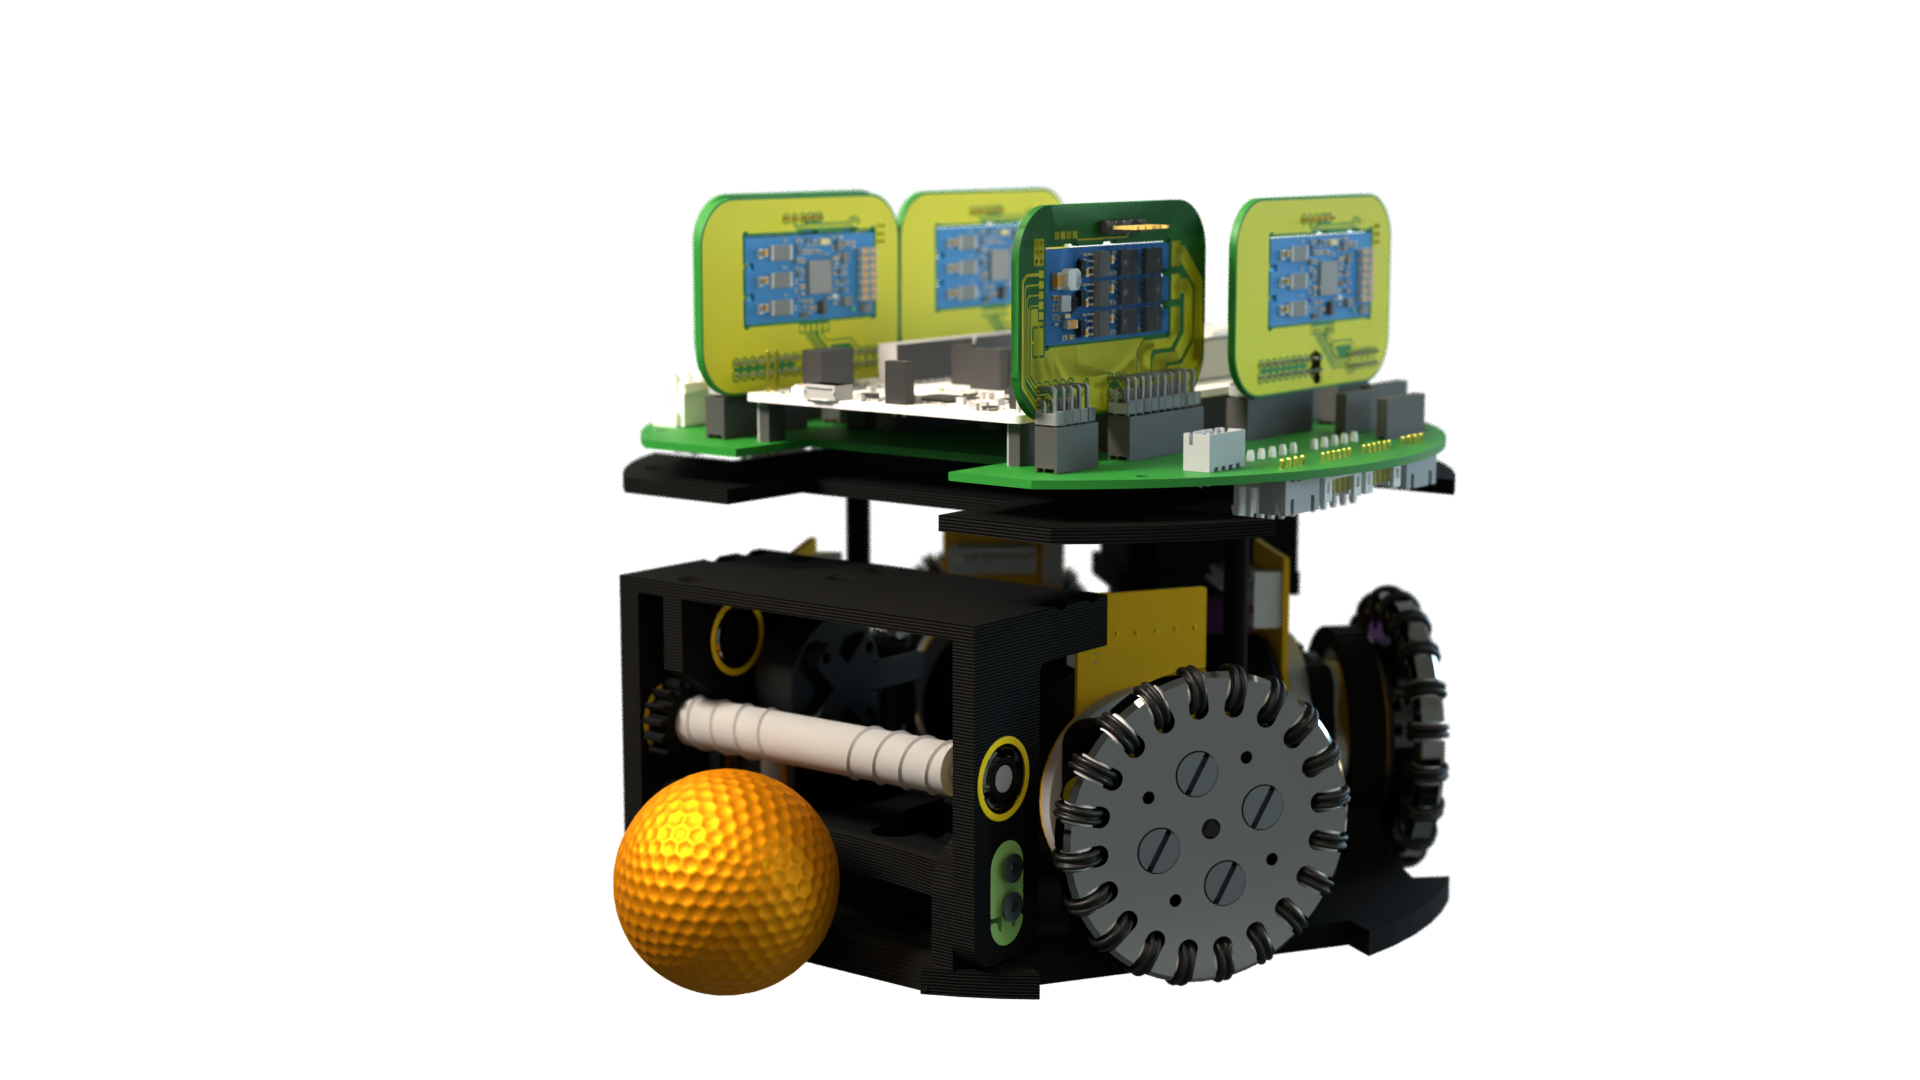
\includegraphics[width=0.5\linewidth]{images/robot_base.png}
	\caption{The constructed robot platform.}
	\label{fig:robot_base}
\end{figure}

%-------------------------------------------------------------------------------
% Electronics
%-------------------------------------------------------------------------------
\subsubsection{Electronics and Power Delivery}
% Intro
The mainboard integrates power delivery, communication between sensors and the \ac{mcu}, and provides connections for the inverters (\hyperlink{bom:B-G431B-ESC1}{B-G431B-ESC1}). Additionally an adapter board for the inverter was designed and manufactured to minimize space usage.
% Power delivery
The robot has components that requires 2.8 \ac{v}, 3.3 \ac{v}, 5 \ac{v} and 24 \ac{v}. Switching regulators are used to step down the battery voltage from 24 \ac{v} to 2.8 \ac{v}, 3.3 \ac{v}, and 5 \ac{v}.

% Circuit safety
The mainboard circuit includes reverse voltage protection, using a hot swap voltage controller.
% ORing circuitry
Two power inputs connected using ORing circuitry is integrated on the mainboard to allow hot swapping the battery.

% Adapter board
Mounting the inverters horizontally does not fit within the dimensions of the mainboard, therefore an adapter board for the inverters was designed and manufactured. The adapter board provides 24 \ac{v} power, traces for each motor winding, data lines for the hall sensors and \ac{uart} for sending instructions aswell as a \(4\)-pin \ac{swd} header.

% Status


%-------------------------------------------------------------------------------
% Microcontroller
%-------------------------------------------------------------------------------
\subsubsection{Microcontroller}
% Intro
The heart of the robot is the NUCLEO-H723ZG microcontroller, it sample the data from the sensors, calculates the kinematics of the robot, communicates with the motor drivers.

%-------------------------------------------------------------------------------
% Motor Control
%-------------------------------------------------------------------------------
\subsubsection{Motor Control}
% intro
The motors in the robot are the \(65\) \ac{w} \ac{bldc} \hyperlink{bom:DF45L024048-A}{DF45L024048-A}. The motors rated speed are \(4840\) \ac{rpm} \(\pm 10\%\) and has a good torque efficiency curve. \hyperlink{bom:DF45L024048-A}{DF45L024048-A} has integrated hall sensors that is used for precise motor control through \ac{foc}.
The \ac{bldc} motors (\hyperlink{bom:DF45L024048-A}{DF45L024048-A}) are controlled using an inverter (\hyperlink{bom:B-G431B-ESC1}{B-G431B-ESC1}). The inverter hosts a programmable STM32 microcontroller, capable of running motor control algorithms such as \ac{foc} and 6-step commutation.
% Why
\hyperlink{bom:DF45L024048-A}{DF45L024048-A} and \hyperlink{bom:B-G431B-ESC1}{B-G431B-ESC1} complement each other by providing a quick setup through \ac{st} MC workbench, streamlining the integration with the rest of the components. By offloading the computations and programming to the inverters microcontroller, it acts as an independent component that can be controlled using the NUCLEO-H723ZG, enabling a fast development process, which is a necessity for this project.
% Status
The integration between \hyperlink{bom:DF45L024048-A}{DF45L024048-A} and \hyperlink{bom:B-G431B-ESC1}{B-G431B-ESC1} was successfully implemented, but the communication between the NUCLEO-H723ZG and \hyperlink{bom:B-G431B-ESC1}{B-G431B-ESC1} could not be established using \ac{UART}.

%-------------------------------------------------------------------------------
% Robot kinematics 
%-------------------------------------------------------------------------------
\subsection{Robot kinematics}

%-------------------------------------------------------------------------------
% Individual robot behaviour
%-------------------------------------------------------------------------------

\subsection{Raspberry Pi executable}
% intro
The Raspberry Pi executable, termed individual robot behaviour, handles high level execution of commands sent from the centralised strategy planner. This includes sensor fusion, localization, path planning and aiming before shooting the ball. It is dependent on hardware interfaces to carry out the low level execution afterwards, like activating motors and kicker.

Sensor fusion, localization and path planning is done using the \ac{ros2} library nav2\:\cite{macenski_desks_2023},\cite{macenski_marathon_2020},\cite{merzlyakov_comparison_2021},\cite{macenski_regulated_2023},\cite{macenski_open-source_2024}.
% Reason
The widely used, and well regarded, nav2 library was chosen because of its optimized performance\:\cite{macenski_desks_2023},\cite{macenski_open-source_2024},\cite{macenski_regulated_2023},\cite{merzlyakov_comparison_2021},\cite{macenski_marathon_2020}, and the quick and easy development that \ac{ros2} and its tools offers, which is necessary given the resources available for this project\:\cite{macenski_robot_2022}.
% Localization
The \ac{amcl} algorithm offered by nav2 was used for localization\:\cite{macenski_desks_2023}. The only parameter that was changed was robot\_model\_type, setting it to nav2\_amcl::OmniMotionModel instead of the default nav2\_amcl::DifferentialMotionModel.
% Sensor fusion
The \ac{ekf} available through nav2 was used for sensor fusion of the \ac{imu} data and wheel encoder data, using only default parameters.
% Global path planning
The default nav2 global path planner, Smac planner (which uses a templated A$^*$, see\:\cite{macenski_open-source_2024}), was used with the default parameters.
% Local path planning
The local path planning was implemented using nav2's DWB method, an expansion of \ac{dwa}\:\cite{macenski_desks_2023}. This package is similar to the original \ac{dwa} method but has been expanded and generalised to also work for omnidirectional platforms by also considering lateral translation, not only forward translation\:\cite{macenski_desks_2023}. It also offers the ability to configure critic functions and trajectory generation, with multiple predefined options made available\:\cite{macenski_desks_2023}. No parameters were changed.
% Computer vision
This part of the system should have object recognition to detect the ball using the available camera on the robot, however this had to be cut because of time constraints.

% Status
Development of this software failed to achieve working status because of limited work force and time.

%-------------------------------------------------------------------------------
% Collective robot behaviour
%-------------------------------------------------------------------------------

\subsection{Centralized Strategy Planner}
For the multi agent decision making, \ac{mappo} is developed for a exploring strategy planning trough \ac{rl}. The use of \ac{rl} is to obtain information from the agent and the environment, learn the correlation between the environment and action. The agents target is to make the best decision according to the state, and gain the maximised reward.
There for \ac{rl} is used to detect new strategy's and efficiently approach unexplored areas. \ac{mappo} is mainly beneficial for \ac{rl} in a multi agent manner. The \ac{mappo} model developed trough a policy and critic network using \ac{rnn} for both networks for decision making and prediction. This model is constructed as a centralised manner, taking the global state provided from GrSim for a global state input for both the policy and critic network. Thus this, the first index in the global state is declared as the robot index to gain knowledge of which agent the policy network is making action decisions on.

\subsubsection{Policy network}
The policy network is built upon the idea of choosing the actions for each agent that will maximize the expected return. By sampling the environment each time step for each episode to acquire state and reward, the policy gradient is then computed in order to update the policy network for maximizing the expected return. The policy network architecture is built as following: The first and second layer are linear layers with tanh as activation functions. Then the output from activation function from the second layer is used as input to the third layer, which is a \ac{gru} layer with the hidden state dimension of 64 units. The last layer will output logits the same dimension as the action space, that will then be used to compute the probability distribution over the actions.

\subsubsection{Critic network}
As the baseline, the on-policy value function was used due to the fact that it reduces variance in the sample estimate for the policy gradient, leading to faster and more stable learning of the optimal policy. The critic network approximates this value function. It estimates the average return the agents get if they start at state $S_t$ and then act according to the current policy for the remainder of the trajectory. The critic network shares the same architecture as the policy network with the same hyper-parameters. Its input shape is dimensioned to fully describe the environment as a global state, which outperforms other representations according to \cite{yu_surprising_2022}.

%Should we put the algorithm here?
\subsubsection{Algorithm}


%-------------------------------------------------------------------------------
% Interfaces, API
%-------------------------------------------------------------------------------

\subsection{Supporting functions}

See Fig.\:\ref{fig:hardware_interface_graph} for a high level overview of how the hardware interface interacts with systems and subsystems.
\begin{figure}
	\centering
	\tikzstyle{block} = [rectangle, rounded corners, minimum width=3cm, minimum height=1cm, text centered, draw=black, fill=gray!20]
\tikzstyle{arrow} = [thick,->,>=stealth]
\tikzstyle{double_arrow} = [thick,<->,>=stealth]

\begin{tikzpicture}[node distance=3cm]

% Nodes
\node (sensors) [block] {Sensor Interface};
\node (nucleo) [block, text width=1.7cm, below of=sensors] {Nucleo 144\newline(\acs{micro-ros})};
\node (raspberry) [block, text width=2cm, right of=nucleo, xshift=3cm] {Raspberry Pi\newline(\acs{ros2})};
\node (wheel) [block, below left of=nucleo, xshift=-2cm] {Wheel Motor Interface};
\node (kicker) [block, below of=nucleo, yshift=-1cm] {Kicker Interface};
\node (dribbler) [block, below right of=nucleo, xshift=2cm] {Dribbler Interface};

% Arrows
\draw [arrow] (sensors) -- (nucleo) node[midway, right] {\acs{i2c}};
\draw [double_arrow] (nucleo) -- (raspberry) node[midway, above] {\acs{ros} over \acs{uart}};
\draw [double_arrow] (nucleo) -- (wheel) node [midway, left, xshift=-0.3cm] {\acs{uart} and \acs{gpio}};
\draw [arrow] (nucleo) -- (kicker) node[midway, right] {\acs{gpio}};
\draw [arrow] (nucleo) -- (dribbler) node[midway, right, xshift=0.3cm] {\acs{pwm}};

\end{tikzpicture}
	\caption{A high level overview of the hardware interface and its interaction with the Raspberry Pi executable.}
	\label{fig:hardware_interface_graph}
\end{figure}

% hardware-Sensors Interface
\subsubsection{Sensor Interface}
To ensure accurate input and output for the robot, multiple sensors were utilized in the hardware interface.

\textbf{\textit{Digital Proximity, Ambient Light, RGB and Gesture Sensor(APDS-9960)}}\\
The APDS-9960 sensor was chosen due to its ability to detect ambient light, proximity, RGB color, and gestures. Our focus was to utilize the proximity detection functionality to detect objects in close proximity to the sensor. The proximity function is useful for RoboCup-Robots as they require interaction with the surrounding environment without direct contact.

The communication was established via I2C interface. The I2C bus allows for efficient data exchange between the sensor and the microcontroller, providing a reliable means of controlling the sensor and retrieving proximity data.

The proximity function of APDS-9960 sensor emit infrared (IR) light and measuring the amount of light that reflects off objects. The reflected light intensity increases when an object enters the proximity range(10 cm) of the sensor.

To establish the communication with the microcontroller STM32 via I2C, the I2C bus uses two wires: The serial data(SDA) and the serial clock(SCL), which allow multiple devices to communicate over the same bus.

To configure the proximity functionality through I2C, we write to the sensor register to configure its operation modes, then we read from a specific registers(See data sheet of APDS-9960).

\subsubsection{IP Communication}


\subsubsection{Automatic Game Controller}


%-------------------------------------------------------------------------------
% Integration
%-------------------------------------------------------------------------------

%-------------------------------------------------------------------------------
\textbf{\textit{MicroRos)}}\\
As a microcontroller, STM32 was chosen for this project. STM32 will be configured as a Micro-ROS node, which will allow interaction with Robot operation system 2 (ROS-2) using the UART communication protocol, making it possible to send and receive ROS-2 messages.
Micro-ROS client libraries are used to successfully publish and subscribe to ROS-2 topics. The UART interface is used as a communication line between STM32 and the Raspberry Pi. UART is chosen because of its simplicity and efficiency for serial communication between embedded devices.

The Raspberry Pi will serve as the central for receiving and processing the data from the STM32, utilizing ROS 2 for higher-level processing and system integration. The Raspberry Pi will also run the Micro-ROS Agent. Which is the communication pipe line between the STM32 and the ROS-2 ecosystem. The Micro-ROS Agent will handle the topics published by the STM32 (Micro-ROS node) and forward them to the corresponding ROS 2 topics on the Raspberry Pi.

\textbf{The process for communication between STM32 and Raspberry pi:}
STM32 sends(publish) sensor data(topics) over UART using the Micro-ROS client. Then the Micro-ROS agent on the Raspberry Pi will receive these topics via the UART interface and forward them to the ROS-2.


\textbf{See Figure [Number of the figure] for deeper understanding}


%===============================================================================

\begin{comment}
In this section you should describe the scientific methods you have used and how you have approached the work itself. For each objective above, identify a method for achieving the objective. The choice of method should be justified. For example, you may have made a mathematical model, used simulations, made an implementation that you tested, or done experiments that you may have evaluated using statistical methods. In the first instance, you should describe the scientific methods you used, but it is also useful to describe how you worked on the task. The Methods section also answers why you did a certain way or why you used a certain tool. So you should not only describe the "what" but also the "why". Ask yourself: can the chosen method help me to achieve the set objectives and thus answer the research question?

Choosing the right scientific method(s) is important for you to achieve your goals \cite{researchmethodology,forskningsmetodik}, so this is a point that you should discuss with your supervisor at an early stage. Also, search the literature for good descriptions of methods, and how best to write a Methods section.
\end{comment}

%===============================================================================

%\newpage
%%===============================================================================
\section{Description of the work}


%===============================================================================

\begin{comment}
After the sections above, there is a description of what you have done. It would help if you did not use the heading above but replaced it with appropriate titles, depending on your work. The structure should be made clear by the section headings. Having a clear, logical structure and a narrative flow is essential. You should include the advanced background knowledge necessary to understand how you solved the assignment and define hypotheses and critical concepts. The description of experiments should be such that it is possible to repeat them. If such a description is very long and detailed, you can put it in an appendix. See below.  
\end{comment}

%===============================================================================
\newpage
%===============================================================================
\section{Results}
\label{section_results}

%-------------------------------------------------------------------------------
% Responsible students
%-------------------------------------------------------------------------------

\textbf{Responsible students: Carl Larsson}

%-------------------------------------------------------------------------------
% Hardware capabilities
%-------------------------------------------------------------------------------

The resulting hardware platform had the capabilities shown in Table.\:\ref{tab:hardware_capabilities}.
\begin{table}[H]
    \centering
    \caption{The hardware capabilities of the constructed robot.}
    \label{tab:hardware_capabilities}
    \begin{tabularx}{\textwidth}{|X|X|} \hline
         \rowcolor{light_grey} \textbf{Metric} & \textbf{Value} \\ \hline
         Max kicking velocity & $3.45$\:\ac{m/s} \\ \hline
    \end{tabularx}
\end{table}
The final cost for one robot was $17319$\:\ac{sek}, but it was not completed within the given time limit of $4$ months.

%-------------------------------------------------------------------------------
% MAPPO
%-------------------------------------------------------------------------------


%===============================================================================

\begin{comment}
Here you can present, for example, the results of experiments, proofs, analysis of data, etc. Your results must be described clearly enough for a reader to be able to judge them.  You should also explain and analyse the results.
\end{comment}

%===============================================================================

\newpage
%===============================================================================
\section{Discussion}
\label{section:discussion}

%-------------------------------------------------------------------------------
% Responsible students
%-------------------------------------------------------------------------------

\textbf{Responsible students: Carl Larsson}

%-------------------------------------------------------------------------------
% Results
%-------------------------------------------------------------------------------

%-------------------------------------------------------------------------------
% Method
%-------------------------------------------------------------------------------

% Priority
Future work is recommended to place more focus on hardware

% Gears
Investigate the use of hypoidgear

% Chassis
Chassis out of carbon fiber

% Dribbler motor
Use smaller dribbler motor

% PCB design
its heavy
A more thorough design without time limitations, allowing for a better board

% Sensors
Use other sensors (lidar, rgb especially) since these were just forced on us and no thought have been put into them. 

% Motor control
Problems with stm ide, DO NOT USE IT
Problems with UART for motors

% Bearing cutout for wheels
Bearing cutouts are not exact since they are cutout by hand

% DWB
DWB has been found to have suboptimal behaviour when its parameters, some of which are interrelated, has not been tuned correctly, which is a complex process\:\cite{macenski_desks_2023}.

% Kicker
The use of linear bearings for the solenoid could help with stability at the cost of taking up more space\:\cite{chen_zjunlict_2018}.

% No global path planning
Global path planning is not strictly necessary for the application of this robot and could be removed (if not for the software stack used) to reduce computational load.

% Stability
Lyapunov tests were not done, hence no part of the system can be guaranteed to be stable\:\cite{borkar_stability_2023}.

% FOC Wizard
Delft did not get \acs{foc} wizard to work.

%-------------------------------------------------------------------------------
% Future work
%-------------------------------------------------------------------------------

% SSL vision problems
\ac{ssl}-vision is unreliable, future work should implement methods which account for and mitigates this\:\cite{huang_zjunlict_2019},\cite{bohm_er-force_2024}.

% Wheel problems
Future work should attempt increasing the number of subwheels to reduce the "polygon effect", Swedish wheels are not perfectly circular but polygonal, becoming more circular as the number of subwheels increase\:\cite{chen_zjunlict_2018}.

% Basestation
No basestation with radio communication, WiFi was used instead which is significantly worse in terms of interference. Future work should focus on developing a good communication system which is not vulnerable to interferance.

% Robot ID
No way of identifying robots was developed, this was left as a future problem to solve.

% More optimal solutions
The use of \acs{slam}-Toolbox is not optimal, future research should investigate more light weight solutions which excludes the use of \ac{slam}

%===============================================================================

\begin{comment}
Here you present the interpretation of the results and assess their significance. Discuss possible implications of the results, and offer possible recommendations. You must report on whether you have achieved the objectives you set out, answering your research question and achieving the aim of your work. The section should also include reflections on the job and its limitations.  You can also discuss solutions to problems that you have identified and discussed earlier or address other issues that the work did not address, questions that were not answered. Also, link your findings to previous work. This way, the discussion can become a conversation with what you wrote in the last section.  Finally, put your work in a broader context, and broaden your perspective. Can your results be generalised? Can what you have done be used in some other context?
\end{comment}

%===============================================================================
\newpage
%===============================================================================
\section{Conclusions}
\label{section:conclusion}

%-------------------------------------------------------------------------------
% Responsible students
%-------------------------------------------------------------------------------

\textbf{Responsible students:}

%-------------------------------------------------------------------------------
% What has been done and what come of it (any noteworhy advances or discoveries)
%-------------------------------------------------------------------------------

%===============================================================================

\begin{comment}
In this section, you should summarise the report and present the conclusions and final analysis. Give a brief overview of the purpose and the research question. You should then clearly state the main findings, explain their significance and put them into context. All conclusions should be supported by previous sections of the report.  However, you should not present new details. 

An expert should be able to read this section independently of the rest of the report. 
\end{comment}

%===============================================================================
\newpage
%===============================================================================
\section*{Acknowledgments}

%-------------------------------------------------------------------------------
% Responsible students
%-------------------------------------------------------------------------------

\textbf{Responsible students: Carl Larsson}

%-------------------------------------------------------------------------------
% Acknowledgement
%-------------------------------------------------------------------------------

% General
The authors would like to thank Emil Persson for their insight throughout the project, as well as  Emil Broberg and Adrian Enrico Mosqueda for their insightful contributions to the research questions.
% Bengt
Special thanks go to Bengt Erik Gustafsson for his guidance on the design and construction of the wheels. 
% Wurth
Finally, the authors acknowledge Filip Agrell and W$\Ddot{\text{u}}$rth for their generous sponsorship of components.

%===============================================================================
\addcontentsline{toc}{section}{Acknowledgments}

% ============================= References ============================

\newpage
% Adjust the bibliography spacing between references to fit IEEEtran
\setlength{\bibsep}{0pt plus 0.3ex}
% abbrvnat is the style for IEEEtran
\bibliographystyle{abbrvnat}
\bibliography{references}
\addcontentsline{toc}{section}{References}

% ============================ Appendices =============================

%\begin{appendices}
	%\input{appendices/appendices1}
	%\clearpage
	%\input{appendices/appendices2}
	%\clearpage
%\end{appendices}

%===============================================================================

\end{document}

%===============================================================================